Mit der Röntgenröhre lassen sich Röntgenemission und unter der Verwendung von Absorbern Röntgenabsorption beobachten.
In beiden Verfahren wird bei der Messung auch Gebrauch der Bragg-Bedingung gemacht.
Dabei trifft Licht unter dem Winkel $\theta$ auf einen Kristall.
\begin{figure}[h!]
  \centering
  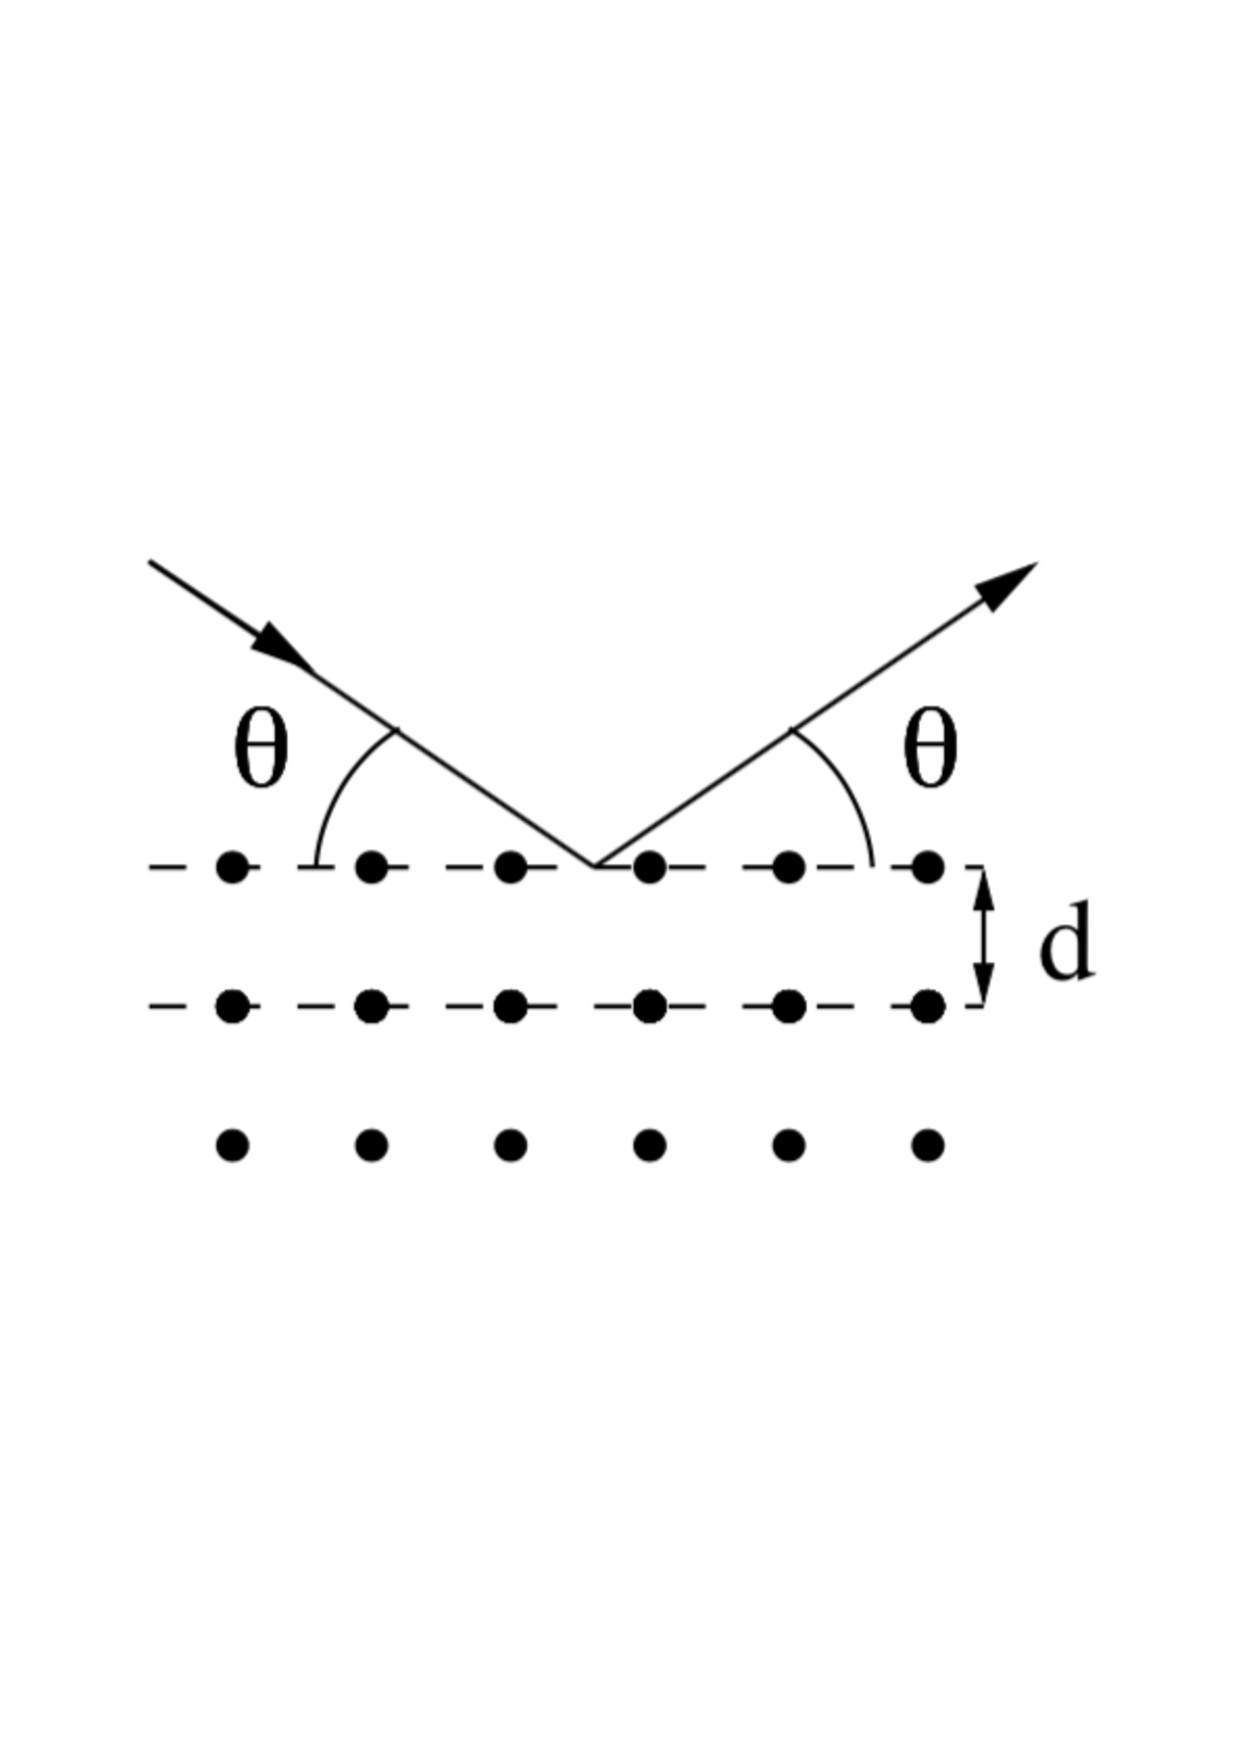
\includegraphics[width=0.6\textwidth]{kristall.pdf}
  \caption{Geometrie der Bragg-Bedingung \cite{1}}
  \label{fig:kristall}
\end{figure}
In dem Kristall sind die Teilchen angeordnet wie in einem dreidimensionalen Gitter (Abb. \ref{fig:kristall}) mit dem Netzebenenabstand $d$.
Das Licht dringt eine oder mehrere Atomschichten in das Material ein, bevor es reflektiert wird.
Es kommt zu einem Gangunterschied $n$ zwischen den oberflächlich reflektierten Wellen und den Wellen, die in den Kristall eingedrungen sind.
Die Wellen interferieren und über die Gleichung
\begin{equation}
  n \lambda = 2 d \sin{\theta} \Leftrightarrow \theta = \arcsin{\frac{n \lambda}{2d}}
  \label{eqn:winkel}
\end{equation}
lässt sich der Glanzwinkel $\theta$ oder die Wellenlänge $\lambda$ berechnen.
In der Messung wird der Winkel des Kristalls verändert um die Intensität der verschiedenen eingestrahlten Wellenlängen kenntlich zu machen.
\FloatBarrier
\subsection{Röntgenemission}
Die Röntgenemission entsteht durch die Beschleunigung von Elektronen zu einer Anode in einem luftleeren Raum und das anschließende Abbremsen der Elektronen im Kernpotenzial.
Die kinetische Energie $E$ eines freien Elektrons im homogenen elektrischen Feld berechnet sich zu:
\begin{equation*}
  E=e_{0} \cdot U.
\end{equation*}
Dabei ist $e_{0}$ die Elektronenladung, $U$ ist die zwischen Kathode und Anode angelegte Spannung.
Die negativ geladenen Elektronen bremsen beim Eintreten in das Potenzial der positiv geladenen Atomkerne des Anodenmaterials ab.
Beim Abbremsen geben die Elektronen ihre kinetische Energie als Strahlung frei.
Die Energie einer elektromagnetischen Welle lautet:
\begin{equation}
  E=h \cdot \nu = \frac{h\cdot c}{\lambda}.
  \label{eqn:lambda}
\end{equation}
$h$ ist das Planck'sche Wirkungsquantum, $\nu$ die Frequenz der Lichtwelle, $\lambda$ ist die Wellenlänge des Lichts und $c$ ist die Lichtgeschwindigkeit.
Die Energien sind gleich, daher gilt:
\begin{equation}
  E=e_{0} \cdot U= \frac{h\cdot c}{\lambda} \Leftrightarrow \lambda=  \frac{h\cdot c}{e_{0} \cdot U}.
\label{eqn:lambdamin}
\end{equation}
Dies gilt jedoch nur für die vollständig abgebremsten Elektronen, daher handelt es sich um die maximale abgegebene Energie.
Die Elektronen sind alle unterschiedlich schnell und geben unterschiedlich viel Energie, also unterschiedliche Wellenlängen, ab.
Dadurch entsteht ein kontinuierliches Spektrum der Röntgenstrahlung (Abb. \ref{fig:kontinuierlich}).
\begin{figure}[h!]
  \centering
  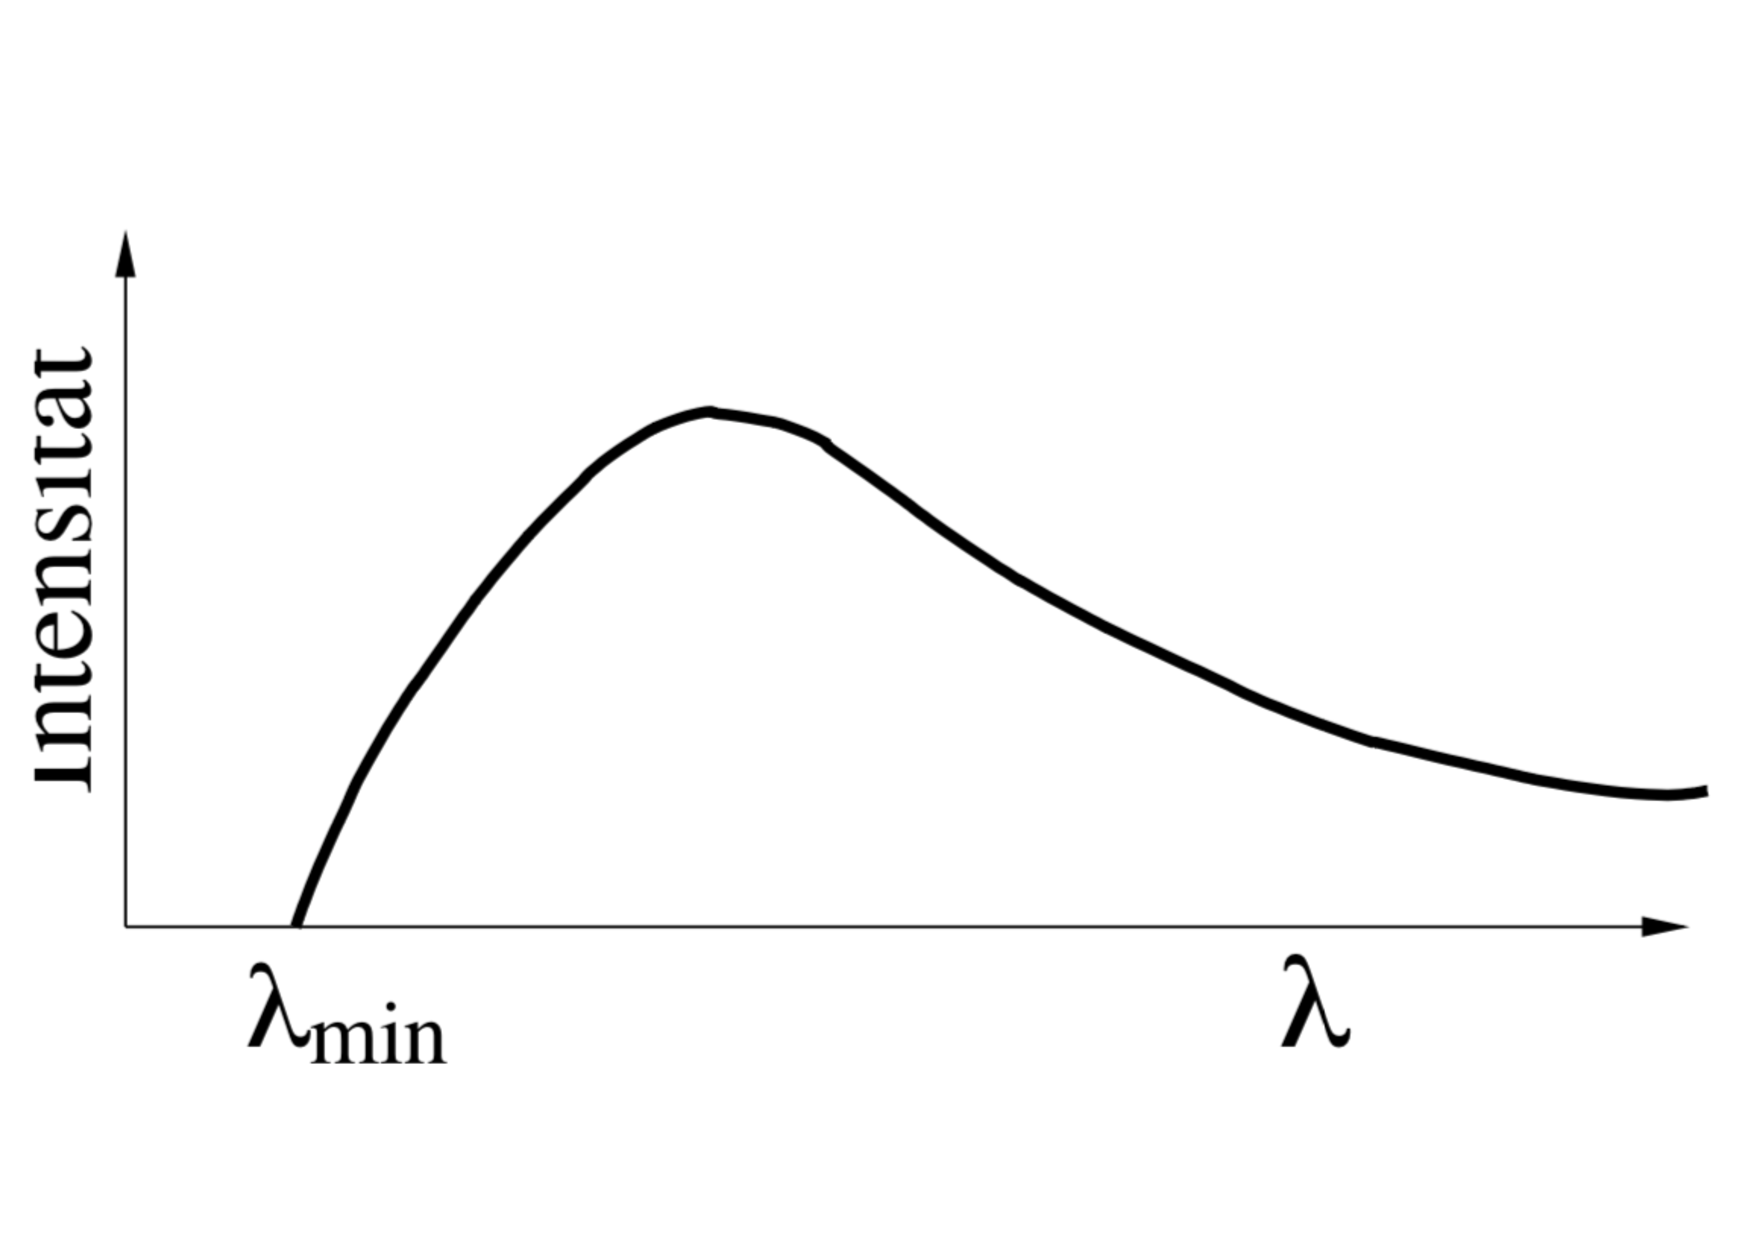
\includegraphics[width=0.8\textwidth]{kontinuierlich.pdf}
  \caption{Kontinuierliches Spektrum der Röntgenemission \cite{1}}
  \label{fig:kontinuierlich}
\end{figure}
\\Zusätzlich zu dem kontinuierlichem Spektrum ergibt sich ein charakteristisches Spektrum.
Dieses entsteht durch die Ionisation der Atome im Anodenmaterial und anschließende Emission der materialspezifischen Röntgenstrahlung.
Dabei schlagen die beschleunigten und abgebremsten Elektronen ein atomeigenes Elektron aus den inneren Energieniveaus.
Das Ausschlagen aus höheren Niveaus ist auch möglich, aber weniger wahrscheinlich.
Die Lücke auf dem innersten Enerieniveau wird von einem Elektron höherer Energieniveaus gefüllt.
Es fällt auf das innerste Niveau und sendet dabei die Energiedifferenz der Niveaus als Röntgenstrahlung aus.
Das innerste Energieniveau wird auch K-Schale genannt, das nächsthöhere Niveau L-Schale.
Die "lückenfüllenden" Elektronen aus verschiedenen Energieniveaus werden durch die griechischen Buchstaben $\alpha, \beta,...$ unterschieden.
So gibt es beispielsweise $K_{\alpha}$- oder $L_{\beta}$-Übergänge, die durch spezifische Energien unterschieden werden können.
\\Die äußersten Elektronen an einem Atom werden durch die negativen Ladungen der Elektronen von der Bindung des positiven Atomkerns abgeschirmt.
Dabei verringert sich die Bindungsenergie der äußeren Elektronen.
Für ein Elektron der n-ten Schale berechnet sie sich durch die Rydbergenergie $E_{Ry}=\SI{13.6}{eV}$ und die effektive Kernladungszahl $Z_{eff}$:
\begin{equation*}
  E_n= - \frac{E_{Ry}\cdot Z_{eff}^2}{n^2}.
\end{equation*}
Die Gleichung lässt sich unter der Beziehung mit der Kernladungszahl $Z$ und der Abschirmkonstanten $\sigma$:
\begin{equation*}
  Z_{eff}=Z-\sigma
\end{equation*}
umstellen nach dem elektronenspezifischen $\sigma$:
\begin{equation}
  E_n= - \frac{E_{Ry}\cdot Z_{eff}^2}{n^2} = - \frac{E_{Ry}\cdot (Z-\sigma)^2}{n^2} \Leftrightarrow \sigma= Z-n\sqrt{\frac{E_{n}}{E_{Ry}}}.
  \label{eqn:E}
\end{equation}
Die Energie eines Übergangs eines Elektrons aus der zweiten Schale ($\alpha$, $n=2$) auf die erste Schale (K, $n=1$) ergibt sich dann zu:
\begin{align}
  E_{K_{\alpha}}&= - \frac{E_{Ry}\cdot (Z-\sigma_{2})^2}{2^2} - \left( - \frac{E_{Ry}\cdot (Z-\sigma_{1})^2}{1^2} \right)\\
  &= E_{Ry} \left(\frac{(Z-\sigma_{1})^2}{1^{2}} - \frac{(Z-\sigma_{2})^2}{2^{2}} \right) .
  \label{eqn:E2}
\end{align}
Die Übergangsenergien lassen sich nicht nur durch die betreffende Schale und die Herkunft des Elektrons genauer differenzieren, es gibt außerdem noch eine feinere Aufspaltung, die sogenannte Feinstruktur und Hyperfeinstruktur.
Sie entsteht durch mehrere Faktoren, zum Beispiel durch die Spin-Bahn-Kopplung der Elektronen, den Elektronenspin, den Lambshift und den Kernspin.
Die Bindungsenergie eines Elektrons unter Beachtung der Feinstruktur lässt sich wie folgt beschreiben:
\begin{equation*}
  E_{n, j}=- E_{Ry} \left[\frac{Z_{eff, 1}^2}{n^2}+\frac{\alpha^2 Z_{eff, 2}^2}{n^3}\left( \frac{1}{j+\frac{1}{2}} - \frac{3}{4n} \right) \right].
\end{equation*}
Dabei ist $n$ die Hauptquantenzahl, $\alpha$ die Sommerfeld'sche Feinstrukturkonstante und $j$ der Gesamtdrehimpuls.
\FloatBarrier
\subsection{Röntgenabsorption}
Bei der Absorption der Röntgenstrahlung kommen bei Energien bis $\SI{1}{MeV}$ meist der Comptoneffekt und der Photoeffekt vor.
Bei dem Comptoneffekt geben die Röntgenquanten einen Teil ihrer Energie mithilfe eines elastischen Stoßes an die schwach gebundenen Elektronen ab.
Da sich die Energie verringert wird die Wellenlänge der Röntgenstrahlung nach dem Stoß größer.
Bei dem Photoeffekt absorbieren die Atome die volle Energie einer vorhandenden Röntgenstrahlung und es werden Elektronen ausgeschlagen.
Beiden Effekten liegt ein Absorptionskoeffizient zugrunde.
\begin{figure}[h!]
  \centering
  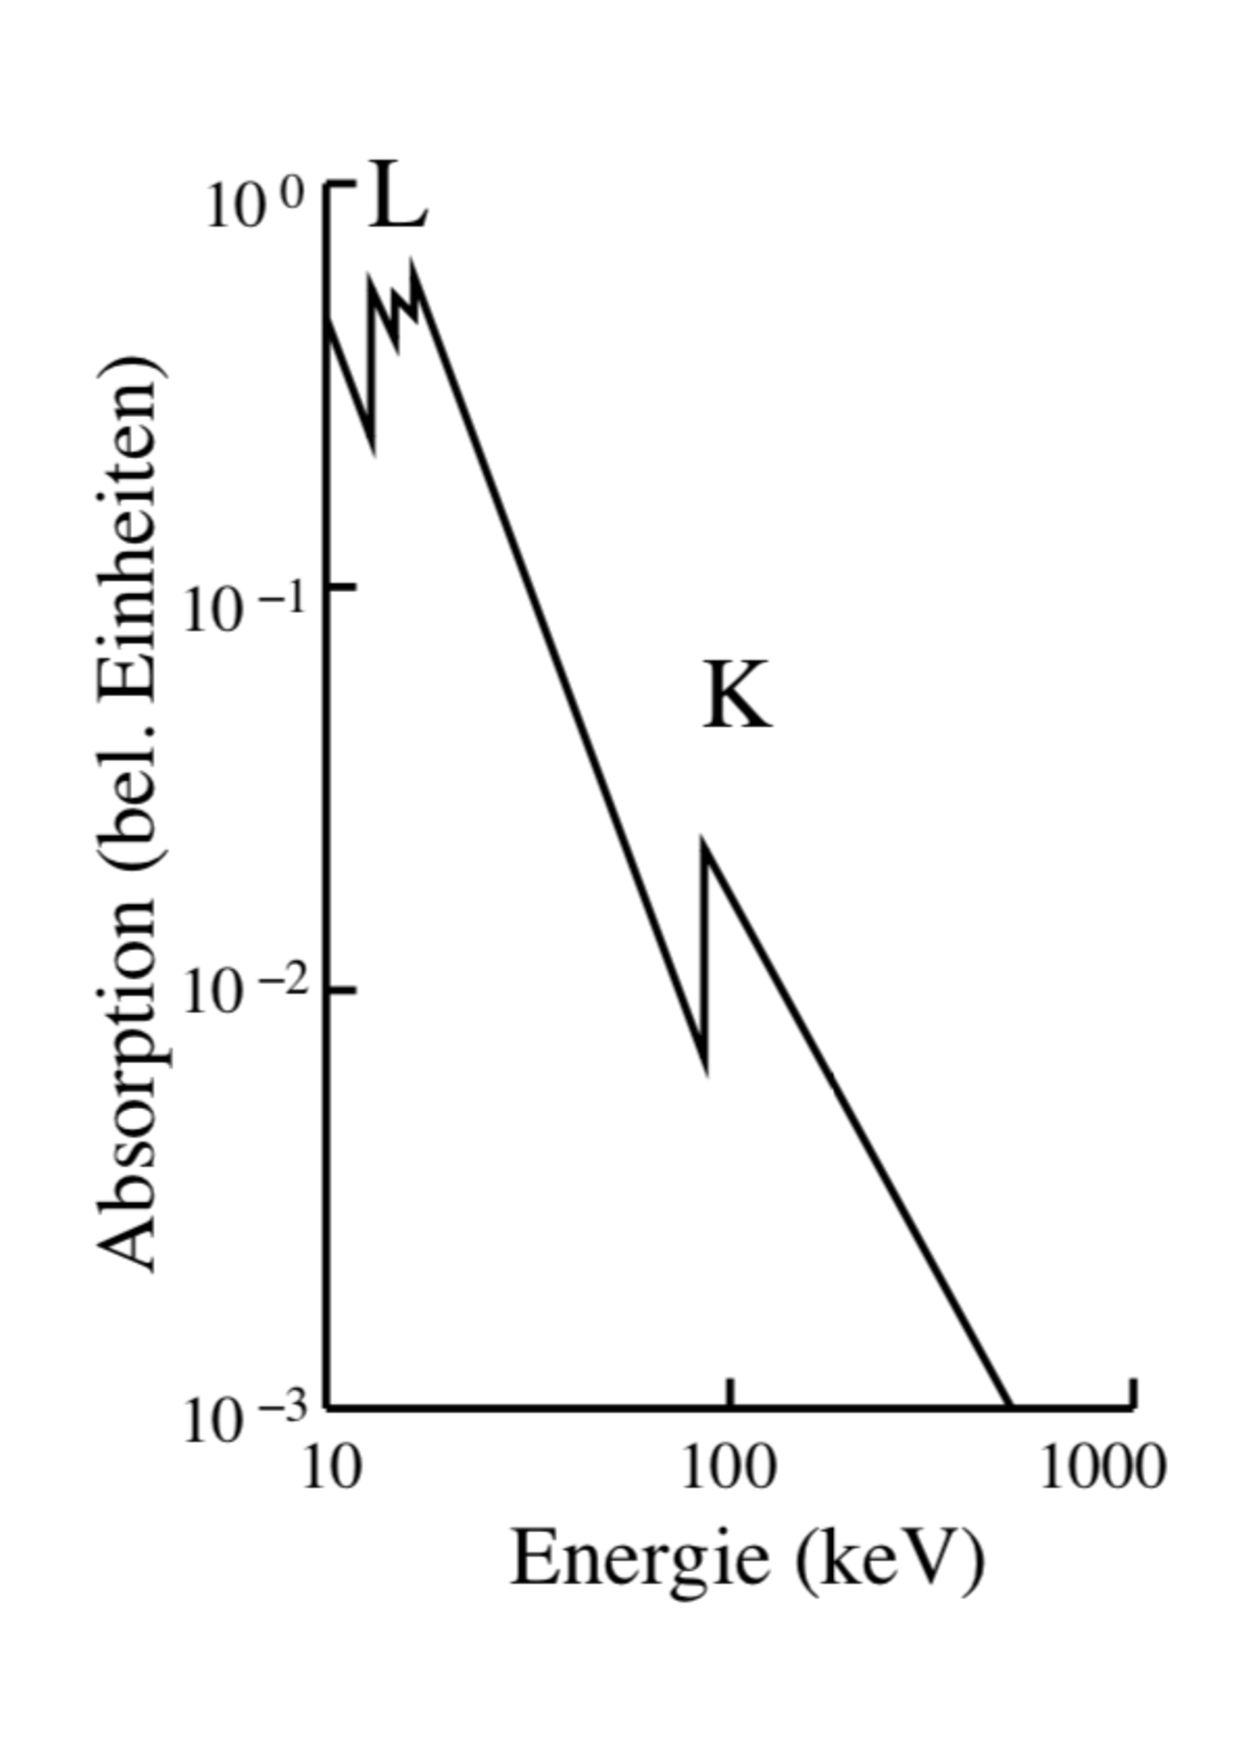
\includegraphics[width=0.5\textwidth]{absorption.pdf}
  \caption{Absorption in Abhängigkeit der Energie der Röntgenquanten \cite{1}}
  \label{fig:absorption}
\end{figure}
Der Absorpionskoeffizient fällt nicht konstant, sondern steigt, sobald die Energie der Röntgenquanten die Bindungsenergie der nächsthöheren Schale erreicht (Abb. \ref{fig:absorption}).
Diese "Zacken" in dem Graphen nennen sich entsprechend der Schale K-, L-, M...-Kante.
Es treten stets nur eine K-Kante und drei L-Kanten auf.
Dies kommt durch die Feinstruktur der Atome, die zum Beispiel aus der Spin-Bahn-Kopplung der Elektronen, dem Elektronenspin, dem Lambshift und dem Kernspin entsteht.
Die drei L-Kanten werden durch die Titel $L_{I}$, $L_{II}$ und $L_{III}$ bezeichnet.
Zur Berechnung der Abschirmkonstante $\sigma_{L}$ einer L-Kante lässt sich die Energiedifferenz $\Delta E_{L}$ zweier L-Kanten verwenden:
\begin{equation}
  \sigma_{L}=Z- \left( \frac{4}{\alpha} \sqrt{\frac{\Delta E_{L}}{E_{Ry}}}-\frac{5 \Delta E_{L}}{E_{Ry}} \right)^{\frac{1}{2}} \left(1+ \frac{19 \alpha^2  \Delta E_{L}}{32  E_{Ry}} \right).
  \label{eqn:sigL}
\end{equation}

\FloatBarrier
